\documentclass[a4paper,12pt]{article}
\usepackage [utf8x]{inputenc}
\usepackage[czech]{babel}
\usepackage{graphicx}
\usepackage{amsmath}
\usepackage{siunitx}
\usepackage{xspace}
\usepackage{url}
\usepackage{indentfirst}
\usepackage[margin=22mm]{geometry}
\usepackage{esvect}
\usepackage{ragged2e}
\usepackage{tikz,pgf}
\usepackage{bm}
\usepackage{perpage}
\usepackage{capt-of}

\graphicspath{
	{img/}
	{plots/}
}

\MakeSorted{figure}
\newtoks\jmenopraktika \newtoks\jmeno \newtoks\datum
\newtoks\obor \newtoks\skupina \newtoks\rocnik \newtoks\semestr
\newtoks\cisloulohy \newtoks\jmenoulohy
\newtoks\tlak \newtoks\teplota \newtoks\vlhkost
\jmenopraktika={Měření prvního Townsendova koeficientu}  % nahradte jmenem vaseho predmetu
\jmeno={Radek Horňák, Lukáš Vrána}            
\datum={1. 3. 2022}        % nahradte datem mereni ulohy                           
\rocnik={2.}                  
\semestr={IV.}                 
\cisloulohy={6}    % cislo ulohy           

\begin{document}
	\begin{center}
		{\Large Přírodovědecká fakulta Masarykovy univerzity} \\
		\bigskip
		{\Large \bfseries PRAKTIKUM Z FYZIKY PLAZMATU} \\
		\bigskip
		{\Large \the\jmenopraktika}
	\end{center}
	\bigskip
	\noindent
	\setlength{\arrayrulewidth}{1pt}
	\begin{tabular*}{\textwidth}{@{\extracolsep{\fill}} l l}
		\large {\bfseries Zpracovali:}  \the\jmeno  \hspace{20mm} \large  
		{\bfseries Naměřeno:} \the\datum\\[2.5mm]
		\hline
	\end{tabular*}

\section{Teorie}

Teorie lavin popsaná Townsendem vysvětluje základní ionizační mechanismus elektrického výboje. Mějme dvě paralelní kovové desky a mezi nimi homogenní elektrické pole $E$. Elektrony jsou v poli urychlovány a sráží se s neutrálními částicemi, přičemž může docházet k nepružným srážkám vedoucím k excitaci nebo ionizaci neutrálů. Pokud počet elektronů v místě $x$ označíme $n$, pak podél dráhy d$x$ vznikne ionizačními srážkami d$n$ nových elektronů a platí

\begin{equation}
	dn = n \alpha dx
\end{equation}

kde $\alpha$ je označení pro první Townsendův, někdy nazývaný i ionizační koeficient. Ten vyjadřuje počet ionizačních srážek jednoho elektronu na jednotkové délce. Integrací a následnou úpravou dostáváme vztah

\begin{equation}
	n = n_0 e^{\alpha x}
\end{equation}

kde $n_0$ je počet elektronů v počátečním bodě $x$ = 0. Ionizační koeficient závisí na intenzitě elektrického pole $E$ a na tlaku plynu v aparatuře $p$. Je li $E/p$ dáno, ,můžeme psát $\alpha$

\begin{equation}
	\alpha = p f \frac{E}{p}
\end{equation}

tedy ionizační koeficient je úměrný počtu srážek na jednotku délky. Experimentální výsledky ukazují, že konkrétní závislost $\alpha$ na $E/p$ je ve tvaru

\begin{equation}
	\frac{\alpha}{p} = A e^{-\frac{Bp}{E}} 
\end{equation}

kde $A$ a $B$ jsou konstanty, pro které platí

\begin{equation}
	U_i = B/A
\end{equation}

kde $U_i$ je ionizační potenciál plynu v aparatuře. Hodnotu konstant A a B lze určit experimentálně.

\section{Měření a výsledky}

Aparatura použitá v tomto praktiku schematicky znázorněná na obr. \ref{aparatura}. Její hlavní komponenty jsou zdroj napětí, rotační olejová vývěva, výbojka, jehlový ventil, Piraniho manometr, ampérmetr a voltmetr. Je založená na principu fotoelektrického jevu, rtuťovou výbojkou osvětlujeme hliníkovou rovinnou katodu a produkujeme tak fotoelektrony. Ty jsou urychlovány homogenním elektrickým polem na mřížkovou anodu. Katodu můžeme posouvat a tím měnit dráhu, po níž dochází k ionizaci neutrálů. Do výbojky, kterou čerpáme vakuovou vývěvou, je vpuštěný argon. Tlak se nastavuje jehlovým ventilem a měří Piraniho manometrem. 

Při měření musíme dbát na to, aby ve výbojce nevznikl samostatný výboj.


\begin{figure}[h]
	\centering
	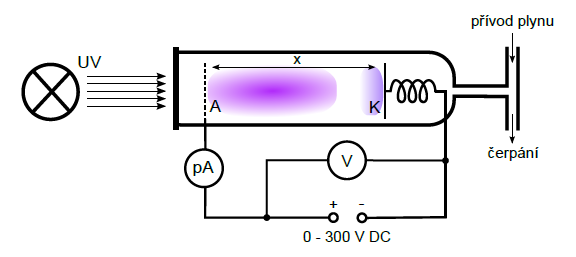
\includegraphics[width=130mm]{aparatura.png}
	\caption{Schéma použité aparatury}
	\label{aparatura}
	\end{figure}

\section{Závěr}


\end{document}
